\documentclass{acm_proc_article-sp}
\usepackage[utf8]{inputenc}
\usepackage{graphicx}
\usepackage{caption}
\usepackage{subcaption}

%opening
\title{An overview of streaming compression techniques}
\numberofauthors{1} 
\author{
% 1st. author
\alignauthor
Benjamin V. Hugo\\
       \affaddr{Department of Computer Science}\\
       \affaddr{University of Cape Town}\\
       \email{bennahugo@aol.com}
}
\begin{document}

\maketitle
\begin{abstract}
 We provide a summary of current compression techniques and their applicability to high volume streaming data. The following techniques are discussed: RLE, 
 Statistical methods such as Huffman and Arithmetic coding, LZ methods, Wavelet Transforms and Predictive Methods for time series. We believe that the compression
 ratios provided by predictive methods, LZ methods and RLE with variable-length coding may yield good results when applied in a context where processing capacity is limited
 due to the shear volume of streaming data received as input.
\end{abstract}

\section{Introduction}
The MeerKAT array outputs very large sets of correlated data (in the area of 1 terabyte per second), making it challenging to distribute and store the data. In light of this, the emphasis of 
this survey will be placed on fast compression techniques that can achieve moderate compression ratios, whilst keeping performance overheads to a minimum.

The concept of compression can ultimately be thought of as expressing information in a more compact form. For example one can eliminate unnecessary information such as repetition 
or encode frequently seen elements using fewer bits. Formally it is expressed as limiting statistical redundancy within data. The techniques for reducing redundancy include the 
following four general methods: run length encoding, statistical methods, LZ methods (dictionary-based) and transforms \cite[p. 7]{salomon2004data}.

It is further important to distinguish between algorithms that are lossless vs. lossy, as well as
those algorithms operating in streaming mode vs. those operating in blocked mode.

An algorithm is said to be lossless when it only encodes information more optimally but does not remove any information.
Lossy algorithms (seen in image compression formats such as JPEG) removes information that 
cannot easily be perceived, but this introduces error in the data \cite[p. 8]{salomon2004data}. For example, the process of scalar 
quantization generally takes large numbers and cuts them down to shorter numbers (this can be done by removing some less 
significant bits) \cite[p. 40]{salomon2004data}. In our context of use we refrain from using these lossy compression techniques due to the 
nature of the correlated radio astronomy data being compressed.

Algorithms operating in blocked mode such as the Burrows-Wheeler algorithm works on input read in large blocks of bytes. Many
encoders, however, work in streaming mode; either a single or a small number of bytes are processed at a time, until the
end of file marker is reached \cite[p. 10]{salomon2004data}.

We also note the following general performance metrics:
 \begin{enumerate}
  \item Compression ratio. A value of 0.6 indicates that the compressed data occupies 60\% of the space of the original, uncompressed
  data. Values greater than 1 indicates negative compression.
  \begin{equation}
   \mbox{Compression ratio} = \frac{\mbox{size of output stream}}{\mbox{size of input stream}} 
  \end{equation}
  \item Compression factor. This is simply the inverse of the compression ratio. Values greater than 1 indicate compression and values less
  than 1 indicate expansion. A bigger value indicates better compression.
  \begin{equation}
   \mbox{Compression factor} = \frac{\mbox{size of input stream}}{\mbox{size of output stream}} 
  \end{equation}
 \end{enumerate}
 
We will first consider some examples in the four main categories before discussing advance techniques focusing on predictive numerical compression.
\section{Run length encoding (RLE)}
In simplest terms run length encoding refers to a simple (and old) scheme of eliminating repetition in runs of characters/bytes: if s = adddddeebbbb then 
RLE(s) = a@d5ee@b4. Usually a special symbol is used to denote a run of symbols. Instead of writing a repeated symbol, say d out 5 times, one can write d5. In light of this RLE is a good candidate for 
instances where information is likely to be repeated \textit{locally} (for instance in image compression). \cite[ch 1]{salomon2004data}.

Ray et al. \cite{ray1995database} investigates several compression techniques for database attribute compression for both text and numerical data. They found that RLE performs well in cases where
there are many redundant characters (as with fixed length string attributes in database tables). However, the compression ratio drops significantly when it is used to compress
real-valued data. Abadi et al. \cite{abadi2006integrating} notes, when testing 32-bit integers, that RLE performs well on low-cardinality data (where there are few discrete values) and 
cases where there are larger run lengths (even for high cardinality data). One can, for instance, encode runs of zero bits in a shorter form if the
numeric data in a scientific database is skewed toward the less significant bits as Bassiouni \cite{1701920} suggests.
\section{Statistical methods}
In Information Theory data redundancy is defined as the difference between the largest possible entropy of a symbol set and its actual entropy. Entropy
is the measurement of the information contained in a single base-n symbol (as transmitted per time unit by some source). Mathematically redundancy is defined 
as follows (n is the size of a symbol set and $P_i$ is the probability that a symbol $c_i$ is transmitted from a source)\cite[p. 46 - 47]{salomon2004data}:
\begin{equation}
 R = \log_2n + \sum_1^nP_i\log_2P_i
\end{equation}
One of the most commonly used algorithms is Huffman coding. It is a form of entropy encoding that compresses data by assigning shorter \textit{integral} representations to symbols that 
occur more frequently \cite[ch 2]{salomon2004data}. Cannane et al. \cite{Cannane:2002:GCS:568727.568730} notes that Huffman coding cannot effectively be applied to cases where words, tokens 
or symbols cannot easily be extracted. These cases includes genome, numeric, scientific and binary formats. 

There is another common entropy encoding technique known as arithmetic encoding. It differs from Huffman coding in the sense that it assigns real-valued intervals to
each symbol (and can therefore more closely match the desired entropy for a particular symbol). The initial interval of [0,1) is refined with the processing of each consecutive character, 
by assigning it to a subinterval within the previous interval. The width of the interval is proportional to the probability with which the character currently being processed occurs \cite[ch 2]{salomon2004data}\cite{Witten:1987:ACD:214762.214771}. 

Both approaches lead to variable-size codes. Both techniques have \textit{adaptive versions} which are useful in situations where the probability distributions change or have to be 
estimated. This approach is also applicable to the situation where the symbol table has to be computed on the fly, because it is impossible to perform multiple passes - as seen with streaming data 
\cite[ch 2]{salomon2004data}\cite{ray1995database}.

A well known example where arithmetic coding is used is in the JPEG2000 image compression standard (known as the MQ algorithm) \cite{952804}. It can, however, also be used for 
numeric compression because it allows for any probability distribution, as pointed out by Witten et al. \cite{Witten:1987:ACD:214762.214771} They add that arithmetic coding is faster than Huffman coding for 
adaptive situations. Analysis performed by Ray et al. \cite{ray1995database} shows that both the adaptive and non-adaptive versions of arithmetic coding produces better 
results than their Huffman counterparts for real-valued data over larger collections. However, it must be pointed out that arithmetic-coding decompression is slow and is not tailored to 
situations where fast access is required \cite{williams1999compressing}.\\

\section{Dictionary (LZ) methods}
Unlike statistical methods, dictionary methods are adaptive methods which do not use variable-size codes. Instead they rely on the recurrences of 
entire phrases. Using a dictionary they encode variable-length phrases to fixed-length codes (hence they resemble entropy encoders in cases where they receive longer input). Two of the primary 
algorithms are LZ77 and LZ78. There are many variants on each of these, including LZSS and LZW. LZ77 uses a sliding window consisting of a search buffer, as well as a look-ahead buffer. The encoder scans
the search buffer backwards trying to locate a match for the characters in the lookahead buffer. The matches are saved as length-distance pairs. LZSS improves upon LZ77 by holding the look-ahead buffer in a circular queue, storing the
dictionary in a binary search tree and constructing tokens with two fields rather than the three-field construction used by LZ77. LZ78 abandons the sliding window approach by keeping a dictionary of strings encountered previously (and can therefore 
use considerable amounts of memory). It is possible to do a two part compression where, for example, LZ77 is followed by a statistical method like Huffman coding (the algorithm is then known as
LZH). The general issue with many of the variants of these algorithms is the size of the dictionary. It can be overcome by breaking the input data into blocks. Below is a short list
of historically popular applications of LZ methods \cite[ch 3]{salomon2004data}:
\begin{enumerate}
 \item The UNIX compress utility and the GIF image format build on a simpler, slow adapting variant of LZ78, called LZW.
 \item The Microsoft ZIP and Cabinet formats
 \item The popular RAR format combines an LZ variant with Huffman encoding.
 \item The compression algorithm known as Deflate combines LZ77 with Huffman encoding. The technique is published in the public domain and is widely used: in the popular 
 UNIX utility GZIP, standard protocols including HTTP and PPP, the PNG image format and Adobe PDF.
\end{enumerate}

Bassiouni \cite{1701920} suggests that LZ methods are primarily used for non-numeric data and are only applicable for header compression in large scientific databases. This notion
is supported by Roth et al. \cite{Roth:1993:DC:163090.163096} They state that LZW achieves very low compression ratios when compressing floating point data (even expansion in the case when the numbers are not 
of the same magnitude). They do however state that data, composed mostly of integers, compress well at around 50\%.

Further analysis by Ray et al. \cite{ray1995database} on a largely numerical database shows that LZ compression achieve lower compression ratios than arithmetic coding if not performed at a file level (ie. 
not on single attributes, records or pages) . However, as previously mentioned, arithmetic coding may be too slow to be employed in our context.

Williams et al. \cite{williams1999compressing} suggests another approach to variable-length representations that work in time-contrained instances where either streaming or random access is required. They show that
variable-length byte schemes constantly outperform LZ-based GZIP's compression ratios for large collections of integers (with both high and low entropies). However, GZIP is consistently
faster than both variable-length byte and bit schemes.

These points raise the possibility of employing an LZ technique such as LZW if the data consists of integers (or floating point numbers in a very limited range), since it is rather fast
and provides support for streaming data.
\section{Wavelet transforms}
A wavelet can, in simple terms, be thought of as an oscillation localized to a finite interval (the amplitude is approximately zero outside the interval). The principle behind wavelet transforms is to transform from a time 
domain to a frequency domain and back. Discreatised wavelet transforms are used in (but not limited to) image and audio compression. The JPEG2000 and DjVu formats are just 2 of the many uses in image formats. The ability to 
decompress a large image progressively in the JPEG2000 standard illustrates why these techniques may be useful \cite[ch 5]{salomon2004data}\cite{952804}. 

In image compression lossless compression can be achieved by combining the discrete wavelet transform known as a Haar transform with RLE and Huffman coding. The Haar transform consists of calculating the averages and differences between 
pairs of samples. The wavelet transform has smaller numbers compared to the values of the original pixels and can therefore be encoded using RLE and Huffman coding \cite[ch 5]{salomon2004data}. Tao et al. 
\cite{Tao:1994:PTS:951087.951108} points out that lossless compression of large collections of scientific floating point data is possible through wavelet transform techniques. However, they are mostly confined to cases where progressive 
transmission between coarse grained and high resolution versions is needed (such as approximate visualizations for large volumes of data and other hierarchical approaches). 
\section{Predictive methods}
It is duly noted that a lot of research is being done on predictive methods and that only a few examples of these techniques are presented. They are context dependent - particularly on the structure of the input data. Some techniques
developed by Engelson et al., Ratanaworabhan et al. and Lindstorm et al. are discussed.

As Engelson et al. \cite{engelson2000lossless} point out: general compression technologies such as text, image and signal compression tools are not intended for use on numerical data of time 
series. There is an opportunity for significant savings, when nearby elements in a time series change only in the least significant bits. Their proposed
algorithm not only work on fixed time steps, but varying time steps as well. They employ a 1D extrapolation of previously received data. The algorithm shows effective compression 
rates when the input data is close to representing some polynomial.

Ratanaworabhan et al. \cite{1607248} suggests a strategy for 64bit floating point compression in time-constrained environments. Their method does not assume that the consecutive
values in a block of data differ only by a small amount as in \cite{engelson2000lossless}. Instead it identifies recurring difference patterns using a hash table lookup, which is then used to make a prediction (using a 
\textit{dfcm} predictor) of the actual value. If the difference between the actual and predicted values are small then the XOR between the two values will contain a large number of leading zeros that can
be compressed using a leading zero count. In particular the sign bits, exponent bits and the first few significant bits of the mantissa in such an XOR will be zero. A performance analysis (in terms of speed) of their compressor, 
(labeled dfcm) is shown in figure \ref{Ratanaworabhan2}. It is interesting to note that their tailored algorithm is much faster than the standard LZ derivatives. In latter works \cite{4589203} they presented an similar algorithm that achieves
even higher throughput.
\begin{figure}[h]
 \centering
 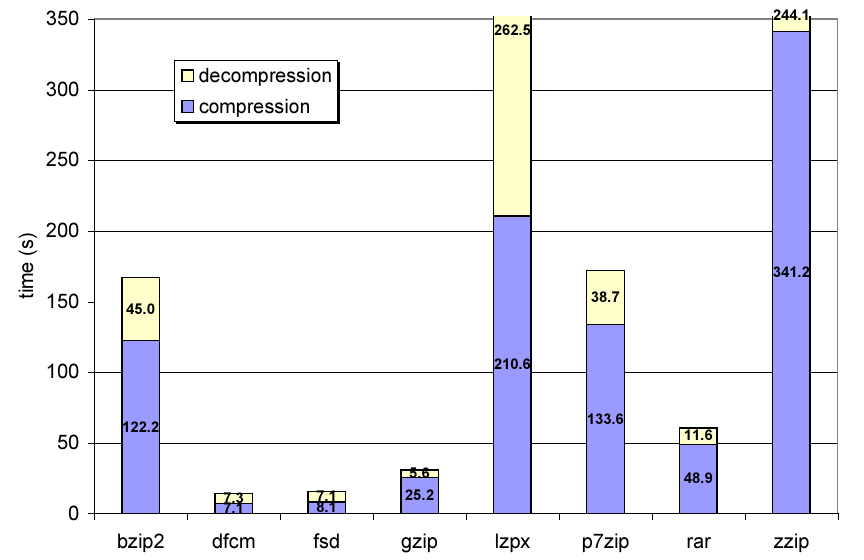
\includegraphics[width=0.48\textwidth]{RatanaworabhanEtAlPerformance.png}
 \caption{Compression/Decompression speed of Ratanaworabhan, Ke and Burtscher's algorithm (dfcm)\cite{1607248}}
 \label{Ratanaworabhan2}
\end{figure}

Taking a different approach to prediction, Lindstrom and Isenburg proposes an online, fast and lossless technique for less structured data than that of Ratanworabhan et al. \cite{lindstrom2006fast} The algorithm 
uses a \textit{Lorenzo} predictor and partitions residuals into entropy codes. The encoder achieves compression ratios comparable to those by Engelson et al., but at twice the speed with a simpler implementation.
They achieve slightly slower compression speeds than those of Ratanaworabhan et al., but with significantly better compression ratios (figure \ref{lindstrom}).
\begin{figure}[h]
 \centering
 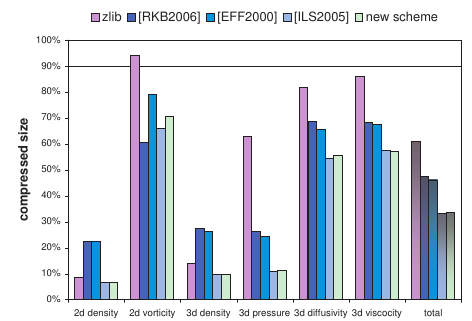
\includegraphics[width=0.48\textwidth]{lindstrom.png}
 \caption{Compression size analysis from lindstrom et al. \cite{lindstrom2006fast}}
 \label{lindstrom}
\end{figure}
\section{Discussion}
In light of the techniques discussed in this literature survey it may be fruitful to try the following techniques: an LZ method such as LZW, predictive methods resembling those
proposed by Ratanaworabhan et al. and RLE with variable length coding (if the data values are skewed towards the least significant bits). Those variable-length coding schemes, based on adaptive arithmetic coding, 
may be too processing intensive for our purposes.
\bibliographystyle{plain}
\bibliography{litRefs}
\end{document}
